\subsection{Signal models considered in this analysis}
\label{subsec:signal_models}
Final states with two same-sign leptons and multiple jets are sensitive to a variety of new physics scenarios. 
In supersymmetric models in particular, such final states can be produced in the decays of heavy superpartners 
involving massive gauge bosons, sleptons or top quarks. 
We list in this section the different simplified models which we used as benchmarks to define our signal regions. 

\begin{figure}[htb!]
\centering
\subfigure{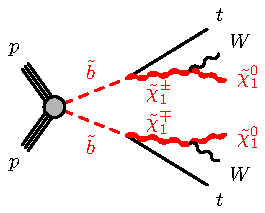
\includegraphics[width=0.24\textwidth]{MODELS/sbsb-ttWWN1N1}}
\subfigure{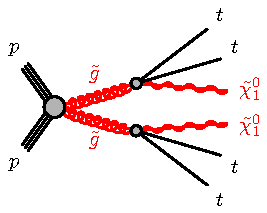
\includegraphics[width=0.24\textwidth]{MODELS/gogo-ttttN1N1}}\hspace{3cm}
\caption{SUSY signal benchmarks leading to multiple $b$-jets : 
direct sbottom pair production decaying to top $+$ chargino (left), and gluino decay via offshell stop (right).}
\label{fig:feynman_3rdgen}
\end{figure}

\begin{figure}[t]
\centering
\subfigure{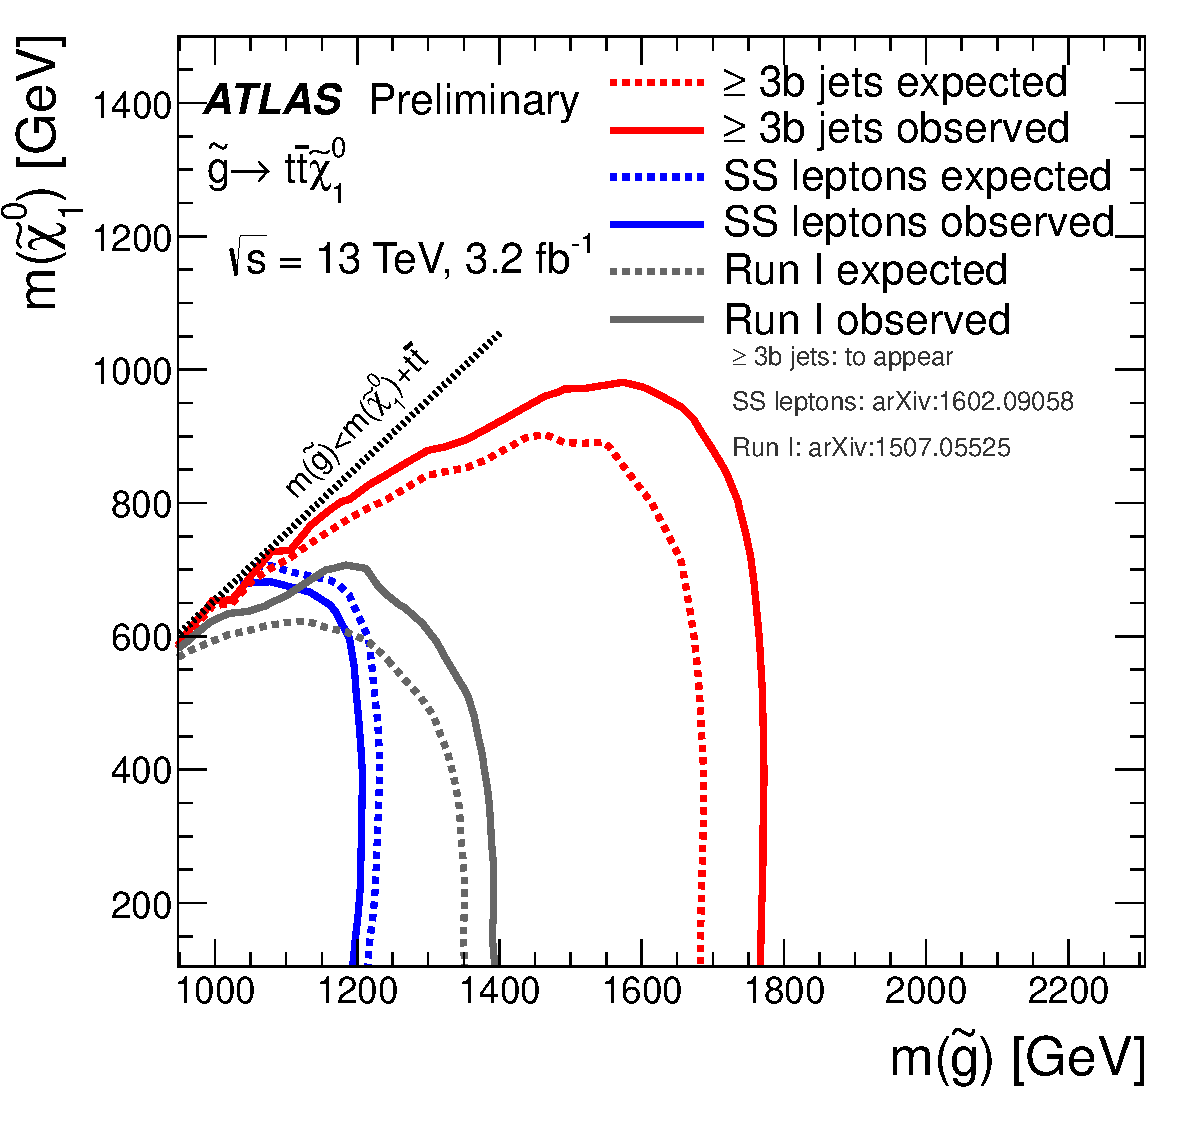
\includegraphics[width=0.49\textwidth]{MODELS/ATLAS_SUSY_Gtt}}
\subfigure{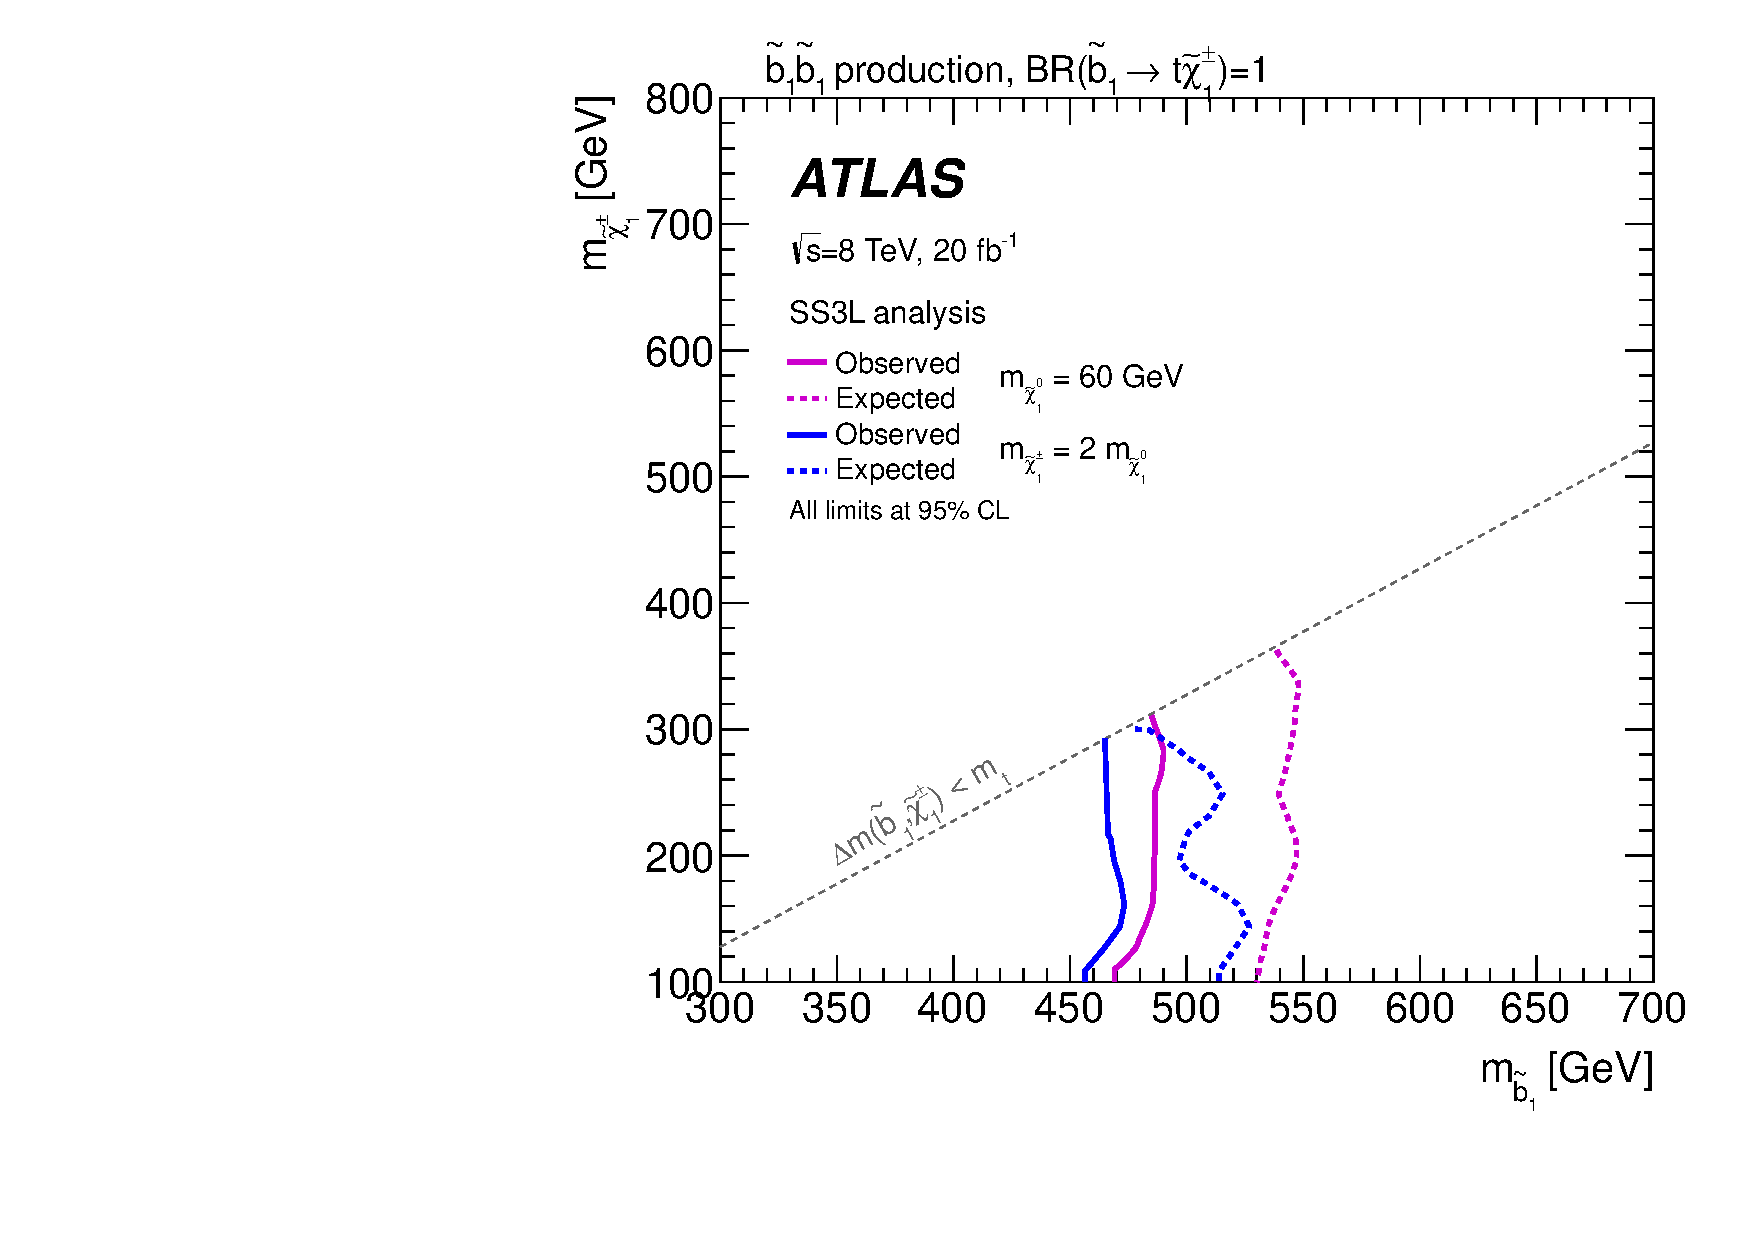
\includegraphics[width=0.49\textwidth]{MODELS/exclusion_sbottom_topC1_both_grids}}
\caption{Exclusion limits on the gluino-stop offshell (left) and direct sbottom (right) scenarios 
set by ATLAS with the 2012 dataset~\cite{DraftSquarkGluinoSummaryPaper}.}
\label{fig:run1excl_3rdgen}
\end{figure}


\par{\bf Direct sbottom $\sbot\to t\chargino$\\}
In this model, bottom squarks are rather light and assumed to decay in a top quark and a chargino $\chargino$ (Fig.~\ref{fig:feynman_3rdgen}), 
providing complementarity to the mainstream search which focuses on the channel $\sbot\to b\neut$. 
The final state resulting from the production of a sbottom pair contains pairs of top quarks, of $W$ bosons and of neutralinos. 
While this final state may lead to various experimental signatures, 
the model was considered in Run-1~\cite{DraftSquarkGluinoSummaryPaper} 
only by the same-sign leptons and jets search, leading to the exclusion limits presented in Fig.~\ref{fig:run1excl_3rdgen}. 
The signal grid generated with the MC15 configurations adopts different hypotheses on the SUSY mass spectrum than what was retained for Run-1: 
in the latter case two grids were proposed with either a fixed neutralino mass (60 GeV) or a fixed chargino-to neutralino mass ratio (2:1). 
The MC15 grid fixes the chargino-neutralino mass difference to 100 GeV, always allowing on-shell $W$ bosons in the $\chargino\to W\ninoone$ decay. 
The reduced chargino-neutralino mass gap compared to the MC12 grids allows to study signal scenarios with heavy neutralinos, which were not considered previously. 
Only pair production of the lightest sbottom is considered, followed by an exclusive decay in the aforementioned channel. \\

\par{\bf Gluino-stop offshell $\gluino\to t\bar t\neut$\\}
In this model inspired by naturalness arguments, gluinos are coupling preferentially to stops which are lighter than the other squarks. 
Gluinos are however considered lighter than stops, and decay directly into a $t\bar t\neut$ triplet via a virtual stop (Fig.~\ref{fig:feynman_3rdgen}). 
The pair production of gluinos leads to a final state containing four top quarks and two neutralinos. 
This characteristic final state is accessible through various experimental signatures, which is why this model 
is commonly used as a benchmark to compare analyses sensitivities. 
The searches performed with Run-1 data~\cite{DraftSquarkGluinoSummaryPaper}, 
summarized in Fig.~\ref{fig:run1excl_3rdgen}, showed that the same-sign leptons final state is competitive only at large neutralino mass. 
This region of the phase space is consequently given a particular attention in the choice of signal regions described further on. 
In the signal samples referenced in this document, the mass of the lightest stop is fixed to 10~\TeV and is mostly a $\widetilde{t}_R$ state. 
Only gluino pair production is considered, followed by an exclusive decay in the aforementioned channel. 
\\

\begin{figure}[h!]
\centering
\subfigure{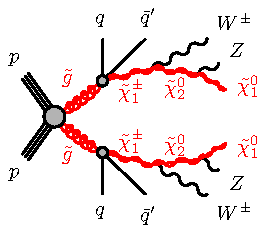
\includegraphics[width=0.24\textwidth]{MODELS/gogo-qqqqWWZZN1N1-C1N2}}\hspace{3cm}
%\subfigure{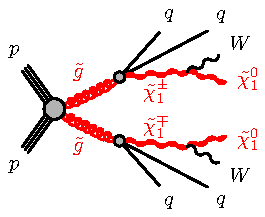
\includegraphics[width=0.24\textwidth]{MODELS/gogo-qqqqWWN1N1}}
%\subfigure{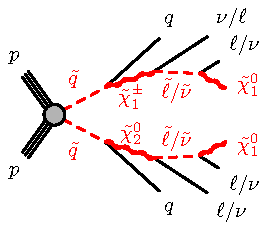
\includegraphics[width=0.24\textwidth]{MODELS/sqsq-qqlllvN1N1-C1N2}}
\subfigure{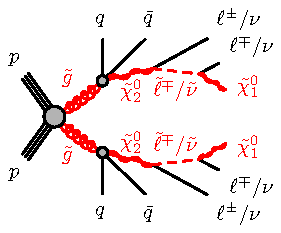
\includegraphics[width=0.24\textwidth]{MODELS/gogo-qqqqllllN1N1-N2}}
%\subfigure{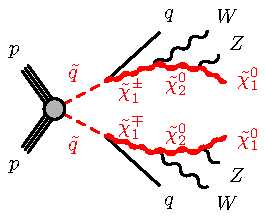
\includegraphics[width=0.24\textwidth]{MODELS/sqsq-qqWWZZN1N1-C1N2}}
\caption{SUSY signal benchmarks leading to no or few $b$-jets : 
gluino pair production followed by two-step decays via heavy gauge bosons or sleptons.}
\label{fig:feynman_1stgen}
\end{figure}

\begin{figure}[t]
\centering
\subfigure{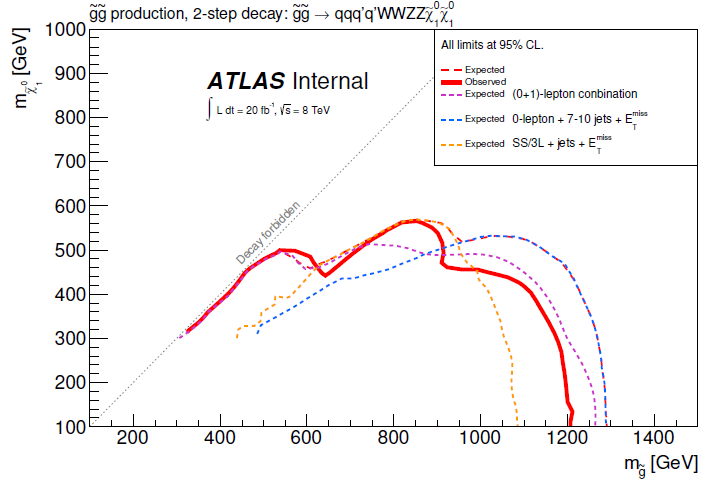
\includegraphics[width=0.49\textwidth]{MODELS/run1excluded_gluino2stepWZ}}
%\subfigure{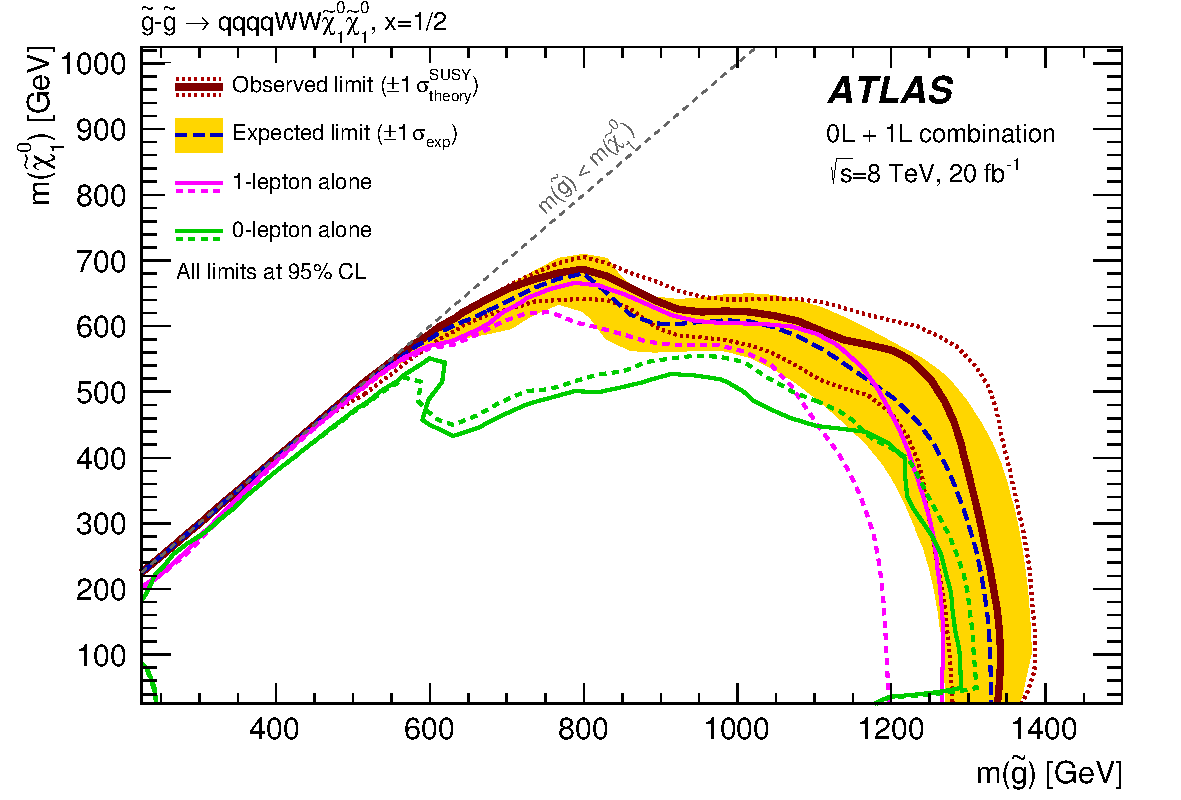
\includegraphics[width=0.49\textwidth]{MODELS/run1excluded_gluino1step}}
\subfigure{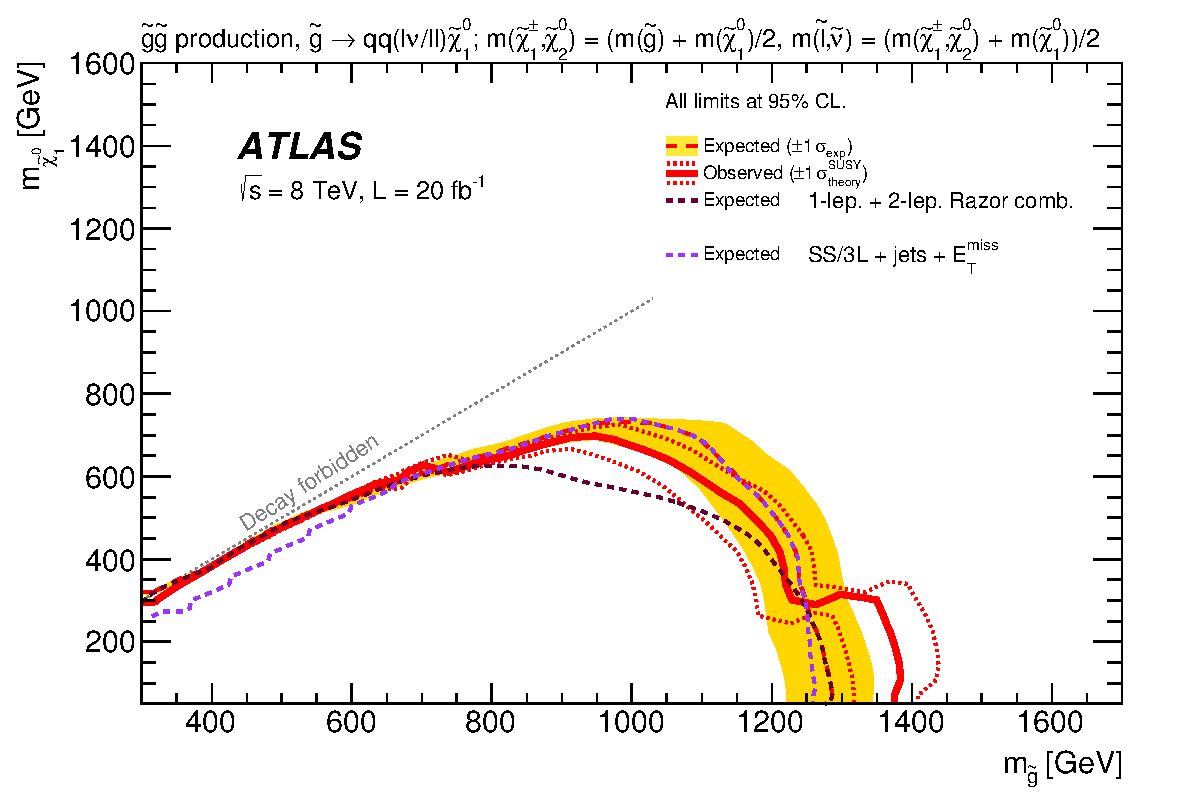
\includegraphics[width=0.49\textwidth]{MODELS/run1excluded_gluino2stepSleptons}}
%\subfigure{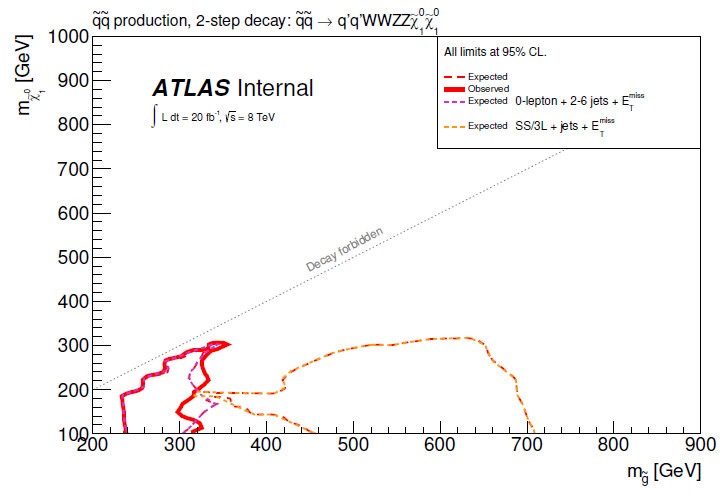
\includegraphics[width=0.49\textwidth]{MODELS/run1excluded_squark2stepWZ}}
%\subfigure{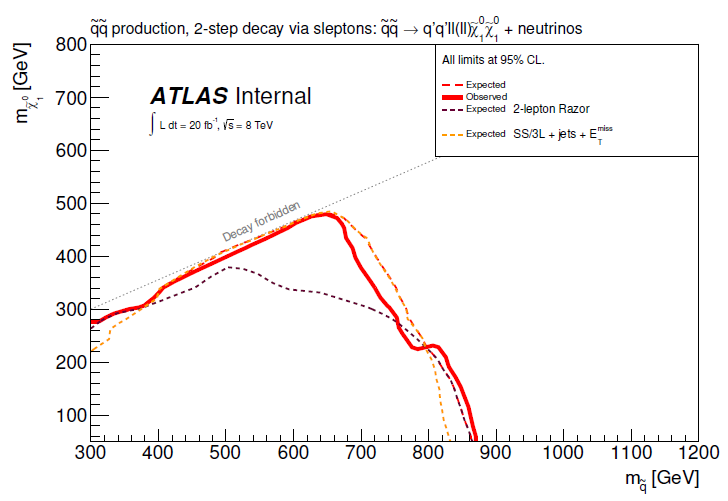
\includegraphics[width=0.49\textwidth]{MODELS/run1excluded_squark2stepSleptons}}
\caption{Exclusion limits on scenarios featuring gluino pair production followed by two-step decays via heavy gauge bosons or sleptons, 
set by ATLAS with the 2012 dataset~\cite{DraftSquarkGluinoSummaryPaper}.}
\label{fig:run1excluded_1stgen}
\end{figure}

%\par{\bf Gluinos and squarks 2-step decays via gauginos\\}
%These scenarios feature a less oriented search for gluinos or squarks (save third generation) where gluinos couple preferentially to the latter, 
%and squarks decay to charginos (Fig.~\ref{fig:feynman_1stgen} left) with the subsequent cascade $\chargino\to W\tilde{\chi}_{2}^{0} \to WZ\neut$. 
%This leads to final states of two light quarks, two $W$ and $Z$ bosons, and two neutralinos 
%(with two additional light quarks in the case of gluino pair production). 
%Fig.~\ref{fig:run1excluded_1stgen} left shows the exclusion limits obtained with the 2012 dataset~\cite{DraftSquarkGluinoSummaryPaper}; 
%in the gluino scenario, the same-sign leptons + jets search provided complementarity at large neutralino mass, 
%while its sensitivity in the squark scenario dominated completely. 
%In the signal samples used here, the chargino mass is set halfway between the neutralino and squark (or gluino) masses, 
%while the neutralino $\tilde{\chi}_{2}^{0}$ mass is set halfway between the chargino and neutralino masses. 
%Gluino and squark-antisquark pair production are considered separately in distinct scenarios.  


\par{\bf Gluinos decays via gauginos\\}
These scenarios feature a less oriented search for gluinos, in the cases when they decay through gauginos in two steps, 
%i.e. by a one-step ($\gluino\to q\bar{q}'\chargino\to q\bar{q}'W\ninoone$) 
either via $W$ and $Z$ bosons ($\gluino\to q\bar{q}'\chargino\to q\bar{q}'W\tilde{\chi}_{2}^{0}\to q\bar{q}'WZ\ninoone$) 
or sleptons ($\gluino\to q\bar{q}'\tilde{\chi}_{2}^{0}  \to  q\bar{q}\ell\tilde\ell/\nu\tilde\nu  \to  q\bar{q}'\ell\ell/\nu\nu\ninoone$). 
The $b$-jet multiplicity in these scenarios is low and they are used as benchmarks to define signal regions with $b$-jet vetoes. 

In the first scenario, the final state is made of two $W$ and two $Z$ bosons (including offshell contributions), 
four additional jets and invisible particles (neutrinos and neutralinos). 
This generally leads to events with large jet multiplicities and a fair branching ratio for dileptonic final states. 
The exclusion limits obtained in run-1 indeed illustrate the competitiveness of the SS/3L+jets search (Fig.~\ref{fig:run1excluded_1stgen} left). 
The signal grid is built with variable gluino and LSP masses, 
and the chargino and neutralino 2 masses are set such that the former lies half-way between the gluino and LSP masses, 
and the latter half-way between the chargino and LSP masses. 

%In the one-step scenario, the final state accessible by this analysis corresponds to four light jets, two leptons, and invisible particles (neutrinos and neutralinos). 
%In run-1, the SS/3L+jets search did not provide competitive limits for this scenario; 
%it is nevertheless interesting to consider in the process of signal region optimization, 
%as it corresponds to less rich event topologies. 
%The signal grid is built with variable gluino and LSP masses, 
%and the chargino mass is set half-way between the gluino and LSP masses. 

In the second scenario, the final state is made of charged leptons, 
four additional jets and invisible particles (neutrinos and neutralinos). 
The average jet multiplicity per event is smaller than in the previous scenario; 
another characteristic is the large fraction of events with several leptons, 
unlike most of the other scenarios that have a rather low acceptance due to the branching ratios of $W\to\ell\nu$ or $Z\to\ell\ell$. 
The exclusion limits obtained in run-1 (Fig.~\ref{fig:run1excluded_1stgen} right) show again that the SS/3L+jets final state 
is very competitive to probe those models. 
The signal grid is built with variable gluino and LSP masses; the $\tilde{\chi}_{2}^{0}$ mass is chosen half-way between the gluino and LSP masses, 
and the sleptons masses are also set equal and half-way between the $\tilde{\chi}_{2}^{0}$ and LSP masses. 
The $\tilde{\chi}_{2}^{0}$ may decay to any of the six sleptons ($\tilde\ell$, $\tilde\nu$) with equal probability. 
Noticeable changes have been introduced with respect to the run-1 grid. 
First, bottom squarks are no longer decoupled but are assumed to be mass-degenerate with the light-flavor squarks, 
opening the decay mode $\gluino\to b\bar b\tilde\chi_2^0$ with $20\%$ branching ratio. 
However, to simplify the model description we do not consider these decay modes; 
this translates concretely into vetoing events with $\gluino\to b\bar b\tilde\chi_2^0$ decays 
and weighting the remaining events by a factor $1/(2*0.2*0.8+0.2^2)$ to readjust the branching ratios. 
Another more important change is that only gluino decays through $\tilde{\chi}_{2}^{0}$ are now considered in the model generation, 
while in the run-1 model decays via charginos $\gluino\to q\bar q'\chargino$ (followed by $\chargino\to\tilde\ell\nu/\ell\tilde\nu$) 
were also considered with a $50\%$ branching ratio. 
The consequences of the latter change are quite important for this analysis, 
reducing the acceptance of inclusive trilepton selections by $\sim 30\%$.  

Since both scenarios include non-resonant $W^*\to\ell\nu$ and $Z^*\to\ell\ell$ contributions, 
they also provide motivated benchmarks to gauge the analysis sensitivity for softer leptons $p_T$ spectra, 
unlike the $\gluino\to t\bar{t}\ninoone$ and $\sbot\to t\chargino$ scenarios 
in which leptons always originate from on-shell $W$ bosons hence can't be arbitrarily soft. 
%\\
%\par{\bf Gluinos and squarks 2-step decays via sleptons\\}
%In these scenarios, gluinos couple preferentially to the squarks of the first two generations, and
%the latter decay either to a chargino $\chargino$ or a neutralino $\tilde{\chi}_{2}^{0}$, 
%which are assumed to be mass-degenerate, and decay in turn to sleptons (Fig.~\ref{fig:feynman_1stgen} right) 
%with $\mathcal{BR}(\chargino\to\nu\tilde\ell) = \mathcal{BR}(\chargino\to\ell\tilde\nu) 
%= \mathcal{BR}(\tilde{\chi}_{2}^{0}\to\nu\tilde\nu) = \mathcal{BR}(\tilde{\chi}_{2}^{0}\to\ell\tilde\ell)=50\%$. 
%The corresponding final state may contain zero to four charged leptons, neutrinos, two light quarks and two neutralinos 
%(with two additional light quarks in the case of gluino pair production). 
%Because of the sleptons replacing the gauge bosons featured in the scenarios presented in the previous paragraph, 
%these scenarios have comparatively a lower jet multiplicity but a significantly enhanced acceptance in multi-lepton experimental signatures. 
%As can be seen on Fig.~\ref{fig:run1excluded_1stgen} right, which presents the exclusion limits obtained with the 2012 dataset~\cite{DraftSquarkGluinoSummaryPaper}, 
%the same-sign leptons and jets signature is again very competitive. 
%In the signal samples used here, the chargino $\chargino$ and neutralino $\tilde{\chi}_{2}^{0}$ masses are set equal, 
%halfway between the neutralino and squark (or gluino) masses, 
%while the degenerate sleptons masses are set halfway between these gauginos and the lightest neutralino masses. 
%Furthermore, gauginos decay to any slepton flavor with equal probability. 
%Gluino and squark-antisquark pair production are considered separately in distinct scenarios. 

\begin{table}
\centering
\resizebox{\textwidth}{!}{
\begin{tabular}{|c|c|c|c|c|c|c|c|c|c|c|}
\hline\hline
Gluino mass (GeV) & 500 & 550 & 600 & 650 & 700 \\\hline
Cross section (pb) & $27.4 \pm 14\%$ & $15.6 \pm 14\%$ & $9.20 \pm 14\%$ & $5.60 \pm 14\%$ & $3.53 \pm 14\%$\\\hline\hline
750 & 800 & 850 & 900 & 950 & 1000\\\hline
$2.27 \pm 14\%$ & $1.49 \pm 15\%$ & $0.996 \pm 15\%$ & $0.677 \pm 16\%$ & $0.466 \pm 16\%$ & $0.325 \pm 17\%$\\\hline\hline
1050 & 1100 & 1150 & 1200 & 1250 & 1300\\\hline
$0.229 \pm 17\%$ & $0.163 \pm 18\%$ & $0.118 \pm 18\%$ & $0.0856 \pm 18\%$ & $0.0627 \pm 19\%$ & $0.0461 \pm 20\%$\\\hline\hline
1350 & 1400 & 1450 & 1500 & 1550 & 1600\\\hline
$0.0340 \pm 20\%$ & $0.0253 \pm 21\%$ & $0.0189 \pm 22\%$ & $0.0142 \pm 23\%$ & $0.0107 \pm 23\%$ & $0.00810 \pm 24\%$\\\hline\hline
\end{tabular}}
\vspace*{0.7cm}
\resizebox{0.8\textwidth}{!}{
\begin{tabular}{|c|c|c|c|c|}
\hline\hline
Sbottom mass (GeV) & 400 & 450 & 500 & 550 \\\hline
Cross section (pb) & $1.84 \pm 14\%$ & $0.948 \pm 13\%$ & $0.518 \pm 13\%$ & $0.296 \pm 13\%$\\\hline\hline
600 & 650 & 700 & 750 & 800\\\hline
$0.175 \pm 13\%$ & $0.107 \pm 13\%$ & $0.0670 \pm 13\%$ & $0.0431 \pm 14\%$ & $0.0283 \pm 14\%$\\\hline\hline
\end{tabular}}

\caption{Signal cross-sections and related uncertainties for scenarios featuring gluino (top table) or sbottom  (bottom table) pair production, 
as a function of the pair-produced superpartner mass, computed in~\cite{Borschensky:2014cia}.}
\label{}
\end{table}

\par{\bf Models not considered for the moment\\}
In the publications~\cite{paperSS3L,DraftSquarkGluinoSummaryPaper} of the analysis results obtained with Run-1 data, 
exclusion limits were also provided for other signal models. 
These scenarios included notably simplified models such as $\gluino\to tbW\neut$, $\gluino\to tcW\neut$, 
squark pair production with similar decay modes as in the previous paragraph, 
as well as minimal models featuring $R$-parity violation through bilinear terms, gauge-mediated SUSY breaking, or universal extra dimensions. 
These models are not considered for the moment, although interpretations might be proposed for them again in the future. 
